\documentclass[11pt]{article}
\usepackage[margin=1in]{geometry}
\usepackage{amsmath,amssymb}
\usepackage{cancel}
\usepackage{xcolor}
\usepackage{booktabs}
\usepackage{array}
\usepackage{longtable}
\usepackage{graphicx}
\usepackage[colorlinks=true,linkcolor=blue,citecolor=blue,urlcolor=blue]{hyperref}

%================================================================
%  The best frequency for inverse-bremsstrahlung heating of krypton laser
%  gases, with a worked example.  C. K. Watson, 12 October 2026.
%  Build: latexmk -pdf envelope_kr_v6.tex
%  The tables (tab_*.tex), fig_v5.pdf and Appendix A (envelope_v6_checks.tex)
%  were generated by the scripts that computed the numbers.  Table rows are
%  read with the TeX primitive \@@input, which works inside a tabular.
%================================================================

\numberwithin{equation}{section}
\setlength{\emergencystretch}{3em}
\setlength{\LTcapwidth}{\textwidth}
\newcolumntype{L}[1]{>{\raggedright\arraybackslash}p{#1}}
\makeatletter
\newcommand{\tabinput}[1]{\@@input #1 }
\makeatother

\newcommand{\ehat}{\hat{\mathbf e}}
\newcommand{\Ev}{\mathbf E}
\newcommand{\vv}{\mathbf v}
\newcommand{\jv}{\mathbf j}
\newcommand{\nuT}{\nu_T}
\newcommand{\nueff}{\nu_{\rm eff}}
\newcommand{\nuea}{\nu_{ea}}
\newcommand{\nuei}{\nu_{ei}}
\newcommand{\num}{\nu_m}
\newcommand{\vt}{v_t}
\newcommand{\dd}{\mathrm d}
\newcommand{\kB}{k_B}
\newcommand{\fbest}{f_{\rm best}}
\newcommand{\Te}{T_e}
\DeclareMathOperator{\Imag}{Im}
\DeclareMathOperator{\Real}{Re}

\title{Detailed derivation of the best frequency\\ for inverse-bremsstrahlung heating\\
of krypton laser gases, with a worked example}
\author{Cooper K.\ Watson}
\date{October 12, 2026}

\begin{document}
\maketitle

\noindent\emph{These notes derive, with every intermediate result written out, the
frequency at which an electromagnetic wave heats the free electrons of a krypton laser
gas best by inverse bremsstrahlung, for two gases, pure krypton and krypton with 2\,\%
fluorine, at electron densities of $10^{14}$ to $10^{16}$~cm$^{-3}$, pressures of 0.1 to
2~atm, and 100 to 500~kW/cm$^3$ deposited for a microsecond. The absorption coefficient
is the Drude form with a collision frequency built from the momentum-transfer cross
sections of the atoms through the two-term kinetic equation, and from the exact
free--free Gaunt factor for the ions. The electron temperature follows from the power
balance, the best frequency from the depth of the gas, the choice between the GHz and the
THz ranges from the absorption across the spectrum, and the uncertainty of the result
from the envelope against a kinetic solution, from the electron--ion term against the
measurements of Turnbull et al., and from the cross sections. A worked example at one
operating point carries the whole chain to a recommended frequency. Every boxed result and
every printed number is checked numerically by} \texttt{envelope\_v6\_check.py}\emph{,
which Appendix~\ref{app:checks} describes.}

\medskip
\noindent For notation, Gaussian units are used in the derivations, as in
\cite{Atzeni2004}, and practical units in the numbers. The electron has charge $-e$ and
mass $m$. The atoms have density $N$ and fractions $x_g$, the electrons density $n_e$ and
temperature $\Te$, the ions density $n_i=n_e$ and charge $e$. The wave has angular
frequency $\omega=2\pi f$ and the field $E_0\cos\omega t$, linearly polarized. The
thermal velocity is $\vt=(\kB\Te/m)^{1/2}$ and the plasma frequency
$\omega_p=(4\pi n_ee^2/m)^{1/2}$. An electron energy is $\varepsilon=mv^2/2$. A boxed
equation is a result that is used later. An equation of another document is cited by
its own number followed by the reference, as in Eq.~(11.9)~\cite{Atzeni2004}, and an
equation number without a reference is one of these notes.

\tableofcontents


%================================================================
\section{The question and what best means}
\label{sec:question}
%================================================================
{\noindent}(1) A wave is to deposit a power $P$ of 100 to 500~kW/cm$^3$ for a microsecond
into the free electrons of a laser gas, of density $n_e=10^{14}$ to $10^{16}$~cm$^{-3}$,
at $p=0.1$ to 2~atm and 300~K, where the gas density is $N=2.45\times10^{19}\,p$
atoms per cm$^3$ per atmosphere. The electrons absorb the wave by inverse
bremsstrahlung, while they collide with the atoms and, far less often, with the ions.
Which frequency does this best?
\\ \\
{\noindent}(2) A wave below the plasma frequency is reflected. A wave just above it is
absorbed in a thin sheet at the front of the gas. A wave far above it crosses the gas and
leaves. The best frequency is therefore the one whose absorption length matches the
depth $L$ of the gas, provided that the gas reflects little of it:
\begin{equation}
\boxed{\;\fbest(L)=\max\big(f_A,f_R\big),\qquad \alpha(f_A)\,L=1,\qquad R(f_R)=5\,\%,\;}
\label{eq:fbest}
\end{equation}
with $\alpha$ the absorption coefficient of the intensity and $R$ the reflection of the
front surface at normal incidence, $f_R$ the lowest frequency that reflects no more than
5\,\%. At $f_A$ one pass absorbs $1-e^{-1}=63\,\%$ of what enters and the deposition at
the back is $e^{-1}$ of that at the front. Asking for $\alpha L=q$ instead moves $f_A$ by
$q^{-1/2}$ where $\alpha\propto f^{-2}$. The reference depth is $L=10$~cm, and
Sec.~\ref{sec:freq} shows $f_A\propto L^{1/2}$.
\\ \\
{\noindent}(3) Two gases are compared: pure Kr, and Kr with 2\,\% F$_2$. The
momentum-transfer and inelastic cross sections are the Biagi set for krypton
\cite{Pitchford2016} and Morgan's set for F$_2$ \cite{Morgan1992}.
\\ \\
{\noindent}(4) The plan. Section~\ref{sec:absorption} derives the absorption coefficient
and the collision frequency of the atoms and of the ions. Section~\ref{sec:temperature}
derives the electron temperature from the power balance, since what the atoms scatter
depends on it. Section~\ref{sec:freq} derives the best frequency in closed form.
Section~\ref{sec:spectrum} follows the absorption across the spectrum and settles the GHz
range against the THz range. Section~\ref{sec:results} gives the results for the two gases
with the particle balance. Section~\ref{sec:kinetic} checks the Maxwellian envelope against
a two-term kinetic solution, Sec.~\ref{sec:uncertainty} derives the uncertainty of every
entry, and Sec.~\ref{sec:example} works one operating point through from the gas density to
the recommended frequency.


%================================================================
\section{The absorption coefficient}
\label{sec:absorption}
%================================================================

\subsection{The Drude model}
\label{sec:drude}
This subsection follows \cite[Sec.~11.1.1]{Atzeni2004}, in whose convention a
perturbation varies as $e^{-i\omega t}$ and the physical quantity is the real part.
\\ \\
{\noindent}(1) The electron velocity obeys Newton's equation with a friction force that
stands for the collisions,
\begin{equation}
-i\omega m\vv=-e\Ev-\nu m\vv
\quad\longrightarrow\quad
\vv=-\frac{e\Ev}{m(\nu-i\omega)}=-\frac{ie\Ev}{m(\omega+i\nu)},
\label{eq:drude-newton}
\end{equation}
which is Eq.~(11.7)~\cite{Atzeni2004}, with $\nu-i\omega=-i(\omega+i\nu)$ in the last step.
\\ \\
{\noindent}(2) The current density and the conductivity are
\begin{equation}
\jv=-en_e\vv=\frac{ie^2n_e}{m(\omega+i\nu)}\,\Ev,\qquad
\sigma=\frac{ie^2n_e}{m(\omega+i\nu)}=\frac{e^2n_e}{m(\nu-i\omega)},
\label{eq:drude-sigma}
\end{equation}
and with the dielectric function $\varepsilon=1+(4\pi i/\omega)\sigma$ of
Eq.~(11.4)~\cite{Atzeni2004},
\begin{equation}
\boxed{\;\varepsilon(\omega)=1-\frac{\omega_p^2}{\omega(\omega+i\nu)}
=1-\frac{\omega_p^2}{\omega^2+\nu^2}+i\,\frac{\omega_p^2\,\nu}{\omega(\omega^2+\nu^2)}.\;}
\label{eq:drude-eps}
\end{equation}
\\ \\
{\noindent}(3) A plane wave $e^{i(kz-\omega t)}$ has $k=(\omega/c)\sqrt\varepsilon$. With
$\sqrt\varepsilon=n_r+i\kappa$ the intensity falls as $e^{-2\Imag k\,z}$, and the
reflection of a sharp boundary at normal incidence is that of the Fresnel formula,
\begin{equation}
\boxed{\;\alpha=\frac{2\omega}{c}\,\kappa,\qquad
R=\Big|\frac{1-\sqrt\varepsilon}{1+\sqrt\varepsilon}\Big|^2.\;}
\label{eq:optics}
\end{equation}
Where the absorption is weak, $\Imag\varepsilon\ll\Real\varepsilon$, one has
$2\kappa\simeq\Imag\varepsilon/n_r$ with $n_r\simeq(\Real\varepsilon)^{1/2}$, so that
\begin{equation}
\boxed{\;\alpha=\frac{\omega}{c}\,\frac{\Imag\varepsilon}{(\Real\varepsilon)^{1/2}}
=\frac{\nu}{c}\,\frac{\omega_p^2}{\omega^2}\Big(1-\frac{\omega_p^2}{\omega^2}\Big)^{-1/2}
\Big[1+O\Big(\frac{\nu^2}{\omega^2}\Big)\Big],\;}
\label{eq:alpha}
\end{equation}
which is Eq.~(11.12)~\cite{Atzeni2004}. Equation~\eqref{eq:optics} is used in the numbers
and Eq.~\eqref{eq:alpha} in the closed forms.
\\ \\
{\noindent}(4) The power absorbed per unit volume is the cycle average of $\jv\cdot\Ev$,
\begin{equation}
\boxed{\;P=\tfrac12\Real\sigma\,E_0^2=\frac{n_ee^2}{2m}\,\frac{\nu}{\omega^2+\nu^2}\,E_0^2.\;}
\label{eq:P-drude}
\end{equation}
Everything that distinguishes one model of inverse bremsstrahlung from another sits in
$\nu$, which the next two subsections build from the collisions with the atoms and with
the ions.

\subsection{The collision frequency of the atoms}
\label{sec:atoms}
{\noindent}(1) In a weakly ionized gas the electrons collide with atoms. The
momentum-transfer collision frequency of an electron of speed $v$ is
$\num(v)=N\sigma_m(v)v$, with $\sigma_m$ the momentum-transfer cross section of the
mixture, $\sigma_m=\sum_gx_g\sigma_{m,g}$. It depends on $v$, strongly so near a
Ramsauer minimum, and the single $\nu$ of Eq.~\eqref{eq:drude-newton} has to be an
average of it with the right weight.
\\ \\
{\noindent}(2) The weight follows from the two-term kinetic equation
\cite{HP2005}. Write the velocity distribution as $f_0(v)+f_1(v)\cos\theta$, with
$\theta$ the angle to the field and $\int4\pi v^2f_0\,\dd v=n_e$. The anisotropic part
obeys, for the field $\Real[E_0\ehat e^{-i\omega t}]$,
\begin{equation}
-i\omega f_1+\num(v)\,f_1=\frac{eE_0}{m}\,\frac{\partial f_0}{\partial v}
\quad\longrightarrow\quad
f_1=\frac{eE_0}{m}\,\frac{\partial_vf_0}{\num(v)-i\omega},
\label{eq:f1}
\end{equation}
where the collisions relax $f_1$ at the rate $\num$ and leave $f_0$ alone.
\\ \\
{\noindent}(3) The current is the first moment of $f_1$,
\begin{equation}
j=-e\int v\cos\theta\,f_1\cos\theta\,\dd^3v=-\frac{4\pi e}{3}\int_0^\infty v^3f_1\,\dd v
=-\frac{4\pi e^2E_0}{3m}\int_0^\infty\frac{v^3\,\partial_vf_0}{\num(v)-i\omega}\,\dd v,
\label{eq:j-lorentz}
\end{equation}
and its real part, which carries the absorption, is
\begin{equation}
\Real\sigma=-\frac{4\pi e^2}{3m}\int_0^\infty\frac{v^3\num(v)}{\num^2(v)+\omega^2}\,\partial_vf_0\,\dd v.
\label{eq:resigma}
\end{equation}
\\ \\
{\noindent}(4) Compare with the Drude form, $\Real\sigma=n_ee^2\nu/[m(\nu^2+\omega^2)]$ from
Eq.~\eqref{eq:drude-sigma}. For $\omega\gg\num$ both denominators are $\omega^2$ and the
comparison defines the effective collision frequency of the atoms,
\begin{equation}
\nuea=-\frac{4\pi}{3n_e}\int_0^\infty v^3\num(v)\,\partial_vf_0\,\dd v.
\label{eq:nuea-general}
\end{equation}
For a Maxwellian, $f_0\propto e^{-v^2/2\vt^2}$ and $\partial_vf_0=-(v/\vt^2)f_0$, so that
\begin{equation}
\boxed{\;\nuea=\frac{\langle\num v^2\rangle}{3\vt^2}
=N\Big\langle\sigma_m v\,\frac{2\varepsilon}{3\kB\Te}\Big\rangle,\;}
\label{eq:nuea}
\end{equation}
the average over the Maxwellian with the energy as a weight: the field heats the fast
electrons most. For a constant $\sigma_m$ this is $4/3$ of the Drude mean
$\langle\num\rangle$, and for the two gases of these notes it is 1.72 to 2.23 times
$\langle\num\rangle$ at the cells of Table~\ref{tab:main} where $\Te\ge0.5$~eV, since
$\sigma_m$ of krypton climbs steeply above its Ramsauer minimum at 0.5~eV. By the low-energy theorem \cite{Low1958,KrollWatson1973} this kernel is exact
for photons of energy small against the electron's, and the atom enters only through
$\sigma_m$.

{\noindent}(5) The same collisions take energy from the electrons. An electron of
energy $\varepsilon$ that scatters elastically through the angle $\chi$ on an atom of mass
$M\gg m$ at rest loses $2(m/M)\varepsilon(1-\cos\chi)$, and the average of
$1-\cos\chi$ over the angular distribution defines $\sigma_m$, so that the loss rate is
$(2m/M)\num(v)\varepsilon$ per electron. Over the Maxwellian, with the gas at $T_g$
giving back $\kB T_g$ for $\kB\Te$,
\begin{equation}
\boxed{\;P_{\rm el}=\sum_gx_g\,\frac{2m}{M_g}\,N\big\langle\sigma_{m,g}v\,\varepsilon\big\rangle
\Big(1-\frac{T_g}{\Te}\Big).\;}
\label{eq:Pel}
\end{equation}

\subsection{The collision frequency of the ions}
\label{sec:ions}
{\noindent}(1) For electrons on ions of charge $e$ the Drude collision frequency is
$\nuei=\nuT\Lambda$ with the Spitzer frequency
\begin{equation}
\boxed{\;\nuT=\frac{4\sqrt{2\pi}}{3}\,\frac{n_ie^4}{m^{1/2}(\kB\Te)^{3/2}}
=2.91\times10^{-12}\,\frac{n_i\,[{\rm m^{-3}}]}{(\kB\Te\,[{\rm eV}])^{3/2}}~{\rm s^{-1}},\;}
\label{eq:nuT}
\end{equation}
which is Eq.~(10.133)~\cite{Atzeni2004} without its logarithm, and $\Lambda$ holds the
physics of the Coulomb collision.
\\ \\
{\noindent}(2) The quantum theory of inverse bremsstrahlung gives $\Lambda$ as a Gaunt
factor. The absorption, net of stimulated emission, of a Maxwellian is
\begin{equation}
\boxed{\;\Lambda=\frac{\pi}{\sqrt3}\,\langle g\rangle(\gamma^2,u)\,\frac{1-e^{-u}}{u},\qquad
u=\frac{\hbar\omega}{\kB\Te},\quad\gamma^2=\frac{{\rm Ry}}{\kB\Te},\;}
\label{eq:Lambda}
\end{equation}
with $\langle g\rangle$ the thermally averaged free--free Gaunt factor of the exact
Coulomb wave functions \cite{KarzasLatter1961}, tabulated by van Hoof et al.\
\cite{vanHoof2014} against $\gamma^2$ and $u$. Its Born limit, $\gamma^2\to0$, is
\begin{equation}
\Lambda_1(u)=\frac{1-e^{-u}}{u}\,e^{u/2}K_0\Big(\frac u2\Big)
\simeq\ln\frac{4\kB\Te}{e^\gamma\hbar\omega}=\ln\frac{b_{\max}}{b_{\min}},\qquad
b_{\max}=\frac{\vt}{\omega},\quad b_{\min}=\frac{e^\gamma}{4}\frac{\hbar}{m\vt},
\label{eq:Lambda1}
\end{equation}
for $u\ll1$, with $\gamma$ Euler's constant in the exponent: the upper cutoff is the
distance an electron travels in a radian of the period, the dynamic cutoff of Dawson and
Oberman \cite{DawsonOberman1962}, which Turnbull et al.\ measured to be the right one
\cite{Turnbull2023}, and not the Debye length.
\\ \\
{\noindent}(3) The Born limit needs $\eta_t=e^2/\hbar\vt\ll1$. Here $\kB\Te$ is about an
electron volt and $\eta_t=3.2$ to 5.3 at the warm cells: the collisions are classical,
and in the soft-photon limit the exact logarithm of one electron is the Born one plus
Bloch's term $-\gamma-\Real\psi(1+i\eta)$, which for $\eta\gg1$ is $-\gamma-\ln\eta$ and
turns the lower cutoff into the classical $e^\gamma e^2/2mv^2$. The tabulated
$\langle g\rangle$ contains this: at the warm cells $\Lambda=2.5$ to 5.6, where the Born
logarithm $\Lambda_1$ would give 3.0 to 7.1.
\\ \\
{\noindent}(4) The two kinds of scatterer add, since electron--ion and electron--atom
collisions are separate events and electron--electron collisions radiate no dipole:
\begin{equation}
\boxed{\;\nueff=\nuea+\nuT\Lambda.\;}
\label{eq:nueff}
\end{equation}
At the cells of Table~\ref{tab:main} with $\Te\ge0.5$~eV, $\nueff=2.7\times10^{11}$ to
$5.7\times10^{12}$~s$^{-1}$, and the ions' share of it is below 2\,\% at $10^{15}$~cm$^{-3}$
and 3 to 26\,\% at $10^{16}$~cm$^{-3}$, the most at 0.1~atm.

\subsection{What is left out, and its size}
\label{sec:leftout}
{\noindent}(1) Screening by the electrons and the correlations of the ions change
$\Lambda$ by a few per cent at most at these densities. (2) The quantum reduction of the
atoms' term at a finite photon energy is below 1\,\% for $u\le0.12$, which holds at every
warm cell. (3) Langdon's flattening of the distribution by the ion heating has the
parameter $\alpha_L=v_{\rm os}^2/\vt^2$ with the quiver velocity $v_{\rm os}=eE_0/m\omega$;
from Eq.~\eqref{eq:P-drude} at $\omega\gg\nu$,
\begin{equation}
\boxed{\;\alpha_L=\frac{v_{\rm os}^2}{\vt^2}=\frac{e^2E_0^2}{m^2\omega^2\vt^2}
=\frac{2\,P/n_e}{\nueff\,\kB\Te},\;}
\label{eq:alphaL}
\end{equation}
where the factor $1+\nu^2/\omega^2$ left out is below 1.06 at the warm cells. It is at most $3\times10^{-3}$ in
Table~\ref{tab:main} wherever the ions carry more than 2\,\% of the absorption, and Langdon's factor \cite{Langdon1980} then changes the
absorption by less than 1\,\% at the warm cells. (4) The reflection is that of a sharp
boundary, an upper bound for a graded one.

\medskip
\noindent\textbf{In Summary:} The absorption coefficient is the Drude form
\eqref{eq:optics} with the collision frequency \eqref{eq:nueff}: the atoms through the
energy-weighted average \eqref{eq:nuea} of their momentum-transfer collision frequency,
exact for soft photons, and the ions through the Spitzer frequency \eqref{eq:nuT} and
the exact Gaunt factor \eqref{eq:Lambda}, whose cutoffs are the dynamic one and the
classical one. Both depend on $\Te$, which the next section fixes.


%================================================================
\section{The electron temperature}
\label{sec:temperature}
%================================================================
{\noindent}(1) The field delivers $P/n_e$ to each electron, and in a steady state the
electrons lose it by elastic recoil, Eq.~\eqref{eq:Pel}, and by the inelastic
collisions with threshold energies $\varepsilon_j$:
\begin{equation}
\boxed{\;\frac{P}{n_e}=P_{\rm el}(\Te)+N\sum_jx_jk_j(\Te)\,\varepsilon_j,\;}
\label{eq:balance}
\end{equation}
which fixes $\Te$ for a Maxwellian. The electrons that attachment removes leave with
their own energy and are replaced by the source that holds the density, so attachment
is not a loss in Eq.~\eqref{eq:balance}. Per electron, $P/n_e$ runs from
$6.2\times10^{7}$~eV/s at $10^{16}$~cm$^{-3}$ and 100~kW/cm$^3$ to $3.1\times10^{10}$~eV/s
at $10^{14}$~cm$^{-3}$ and 500~kW/cm$^3$.
\\ \\
{\noindent}(2) The rate coefficient of a process of cross section $\sigma_j(\varepsilon)$
is $k_j=\langle\sigma_jv\rangle$. With the Maxwellian written in the energy,
$F(\varepsilon)=\frac{2}{\sqrt\pi}(\kB\Te)^{-3/2}e^{-\varepsilon/\kB\Te}$ normalized by
$\int_0^\infty\varepsilon^{1/2}F\,\dd\varepsilon=1$, and $v=\gamma_e\varepsilon^{1/2}$ with
$\gamma_e=(2/m)^{1/2}$,
\begin{equation}
\boxed{\;k_j=\int_0^\infty\sigma_j(\varepsilon)\,v\,\varepsilon^{1/2}F(\varepsilon)\,\dd\varepsilon
=\gamma_e\int_0^\infty\varepsilon\,\sigma_j(\varepsilon)\,F(\varepsilon)\,\dd\varepsilon,\;}
\label{eq:rate}
\end{equation}
and the same weight $\varepsilon F$ gives Eq.~\eqref{eq:nuea} as
$\nuea=N\gamma_e\int\varepsilon\sigma_m(2\varepsilon/3\kB\Te)F\,\dd\varepsilon$ and
Eq.~\eqref{eq:Pel} with $\varepsilon^2\sigma_mF$.
\\ \\
{\noindent}(3) In pure Kr the recoil takes 0.1 to 24\,\% of the power and the 5s
excitation of krypton at 9.9~eV the rest, so $\Te$ sits where the Maxwellian tail reaches
10~eV: 0.95 to 2.6~eV at 300~kW/cm$^3$. With 2\,\% F$_2$ the vibrational channels (0.1 to
0.4~eV) and the dissociative ones (3.2 and 4.3~eV) take 1 to 13\,\% of the losses at
$10^{14}$~cm$^{-3}$, 8 to 74\,\% at $10^{15}$ and 45 to 100\,\% at $10^{16}$, where the
power per electron is least, and lower $\Te$ to 1.05~eV at $10^{15}$~cm$^{-3}$ and 2~atm
and, at $10^{16}$~cm$^{-3}$, to 1.23~eV at 0.1~atm and to 0.19 and 0.088~eV at 0.5 and
2~atm.
\\ \\
{\noindent}(4) At the two cells where F$_2$ holds $\Te$ at 0.19 and 0.088~eV, in and below
the Ramsauer minimum of krypton, the ions carry 79 to 92\,\% of $\nueff$, $u$ reaches 0.30
and 1.0, outside the soft-photon range of the atoms' term, and no source could hold the
electrons (Sec.~\ref{sec:particles}). Their entries in the tables are formal.
\\ \\
{\noindent}(5) The field itself follows from Eq.~\eqref{eq:P-drude} once
$\alpha L=1$ ties the frequency to the collision frequency. With Eq.~\eqref{eq:alpha},
$\nu/(\omega^2+\nu^2)=c\,n_r/(\omega_p^2L)$ at $f_A$, and Eq.~\eqref{eq:P-drude} becomes
\begin{equation}
\boxed{\;E_0=\Big(\frac{8\pi PL}{c\,n_r}\Big)^{1/2}
=47.5~{\rm kV/cm}\,\Big(\frac{P}{300~{\rm kW/cm^3}}\,\frac{L}{10~{\rm cm}}\Big)^{1/2}n_r^{-1/2},\;}
\label{eq:E0}
\end{equation}
the same at every cell but for $n_r$, since the absorbed power per volume is the
intensity over the absorption length: the intensity is $PL$ in that sense, 3~MW/cm$^2$ at
300~kW/cm$^3$ and 10~cm.

\medskip
\noindent\textbf{In Summary:} The power balance \eqref{eq:balance} with the Maxwellian
rates \eqref{eq:rate} sets $\Te$ at 0.95 to 2.6~eV at the warm cells of the two gases.
The 5s level of krypton takes the power in pure Kr, and F$_2$'s low channels take over
where the power per electron is least and cool the electrons into the Ramsauer minimum.


%================================================================
\section{The best frequency}
\label{sec:freq}
%================================================================

\subsection{The reflection limit}
\label{sec:reflection}
{\noindent}(1) For $\nu\ll\omega$ the dielectric function \eqref{eq:drude-eps} is real,
$\varepsilon=1-\omega_p^2/\omega^2$, and above the cutoff $\sqrt\varepsilon=n_r$ is real
too, so that Eq.~\eqref{eq:optics} gives $R=[(1-n_r)/(1+n_r)]^2$. Solving for $R=5\,\%$,
\begin{equation}
n_r=\frac{1-\sqrt R}{1+\sqrt R}=0.6345,\qquad
\boxed{\;\frac{f_R}{f_{pe}}=\big(1-n_r^2\big)^{-1/2}=1.294\quad(\nu\ll\omega_p),\;}
\label{eq:fR}
\end{equation}
with the cutoff $f_{pe}=\omega_p/2\pi=8.98~{\rm kHz}\,(n_e/{\rm cm^{-3}})^{1/2}$, which is
0.090, 0.28 and 0.90~THz at the three densities. So $f_R\le1.16$~THz, at $10^{16}$~cm$^{-3}$.
Where $\nu$ exceeds $\omega_p$, at $10^{14}$~cm$^{-3}$ from 0.5~atm up, the collisions damp
the reflection and $f_R$ falls to 0.03~THz and below, far under $f_A$.

\subsection{The absorption length}
\label{sec:length}
{\noindent}(1) Well above the cutoff and the collision frequency Eq.~\eqref{eq:alpha} is
$\alpha=\omega_p^2\nueff/(c\,\omega^2)$, and $\alpha L=1$ gives
\begin{equation}
\boxed{\;f_A=\frac{1}{2\pi}\Big(\frac{\omega_p^2\,\nueff\,L}{c}\Big)^{1/2}
=5.2~{\rm THz}\Big(\frac{n_e}{10^{15}~{\rm cm^{-3}}}\;\frac{\nueff}{10^{12}~{\rm s^{-1}}}\;
\frac{L}{10~{\rm cm}}\Big)^{1/2},\;}
\label{eq:fA}
\end{equation}
within 3.1\,\% of the exact root of $\alpha L=1$ with Eq.~\eqref{eq:optics} at every one of
the 54 points computed below. At every one of them $f_A>f_R$: the absorption length, not
the cutoff, sets the frequency.

{\noindent}(2) Since $\nueff\simeq\nuea\propto N\sigma_m(\Te)$, the best frequency grows
as the square root of the electron density, of the gas density, and of the depth. The
exponents come out below $1/2$ in the fits of Sec.~\ref{sec:laws}, because the hotter,
thinner cells scatter more per atom: $\Te$ falls with $n_ep$ through
Eq.~\eqref{eq:balance}, and $\sigma_m$ with it.

\medskip
\noindent\textbf{In Summary:} The best frequency is Eq.~\eqref{eq:fA}, the frequency
whose absorption length is the depth of the gas, bounded below by the reflection limit
\eqref{eq:fR}, which never binds here.


%================================================================
\section{The spectrum: GHz or THz?}
\label{sec:spectrum}
%================================================================
{\noindent}(1) Before the best frequency is read off, the whole spectrum is worth a look, since
the microwave sources sit in the GHz range. With each cell's $\nueff$ and $\omega_p$,
Eqs.~\eqref{eq:drude-eps} and \eqref{eq:optics} give $\alpha(f)$ and $R(f)$ from 1~GHz to
100~THz, the ions' logarithm taken at each frequency. Three regimes appear. Below the collision
frequency the wave enters as a collisional skin: with $\omega\ll\nu$ and
$\omega_p^2\gg\omega\nu$, Eq.~\eqref{eq:drude-eps} is dominated by its imaginary part,
$\varepsilon\simeq i\omega_p^2/\omega\nu$, so that
$\sqrt\varepsilon\simeq(1+i)(\omega_p^2/2\omega\nu)^{1/2}$ and
\begin{equation}
\boxed{\;\alpha\simeq\frac{\omega_p}{c}\Big(\frac{2\omega}{\nueff}\Big)^{1/2}\qquad(\omega\ll\nueff),\;}
\label{eq:skin}
\end{equation}
rising as $f^{1/2}$: at 2.45~GHz this law reproduces the exact $\alpha$ within a factor 0.98 to
1.14 at the 18 cells. Near the larger of the collision frequency and the cutoff, $\alpha$ peaks, at
0.05 to 0.50~THz over the 18 cells, and the absorption length is shortest there, 0.03 to 1.7~mm for
pure Kr at 0.5~atm. Above both, the gas is transparent, $\alpha$ falls as $f^{-2}$ by
Eq.~\eqref{eq:alpha}, and $R\to0$. Here $\nueff/2\pi=0.009$ to 0.91~THz and
$f_{pe}=0.090$ to 0.90~THz, so the boundary between the two bands is where the physics turns:
the GHz band lies on the skin side and the THz band on the transparent side.
\\ \\
{\noindent}(2) Table~\ref{tab:spectrum} and Fig.~\ref{fig:spectrum} give pure Kr at 0.5~atm:
the absorption length $1/\alpha$, the reflection $R$, and the fraction
$A=(1-R)(1-e^{-\alpha L})$ of the incident power deposited in the 10~cm.

\begin{table}[ht]
\centering
\caption{Pure Kr at 0.5~atm, from 2.45~GHz to 30~THz: the absorption length, the reflection in
per cent, and the fraction of the incident power deposited in $L=10$~cm, in per cent, at the
three densities.}
\label{tab:spectrum}
\small
\setlength{\tabcolsep}{4.5pt}
\begin{tabular}{lccccccccc}
\toprule
 & \multicolumn{3}{c}{$10^{14}$~cm$^{-3}$} & \multicolumn{3}{c}{$10^{15}$~cm$^{-3}$} & \multicolumn{3}{c}{$10^{16}$~cm$^{-3}$}\\
\cmidrule(lr){2-4}\cmidrule(lr){5-7}\cmidrule(lr){8-10}
$f$ & $1/\alpha$ & $R$ & $A$ & $1/\alpha$ & $R$ & $A$ & $1/\alpha$ & $R$ & $A$\\
\midrule
\tabinput{tab_v5.tex}
\bottomrule
\end{tabular}
\end{table}

\begin{figure}[ht]
\centering
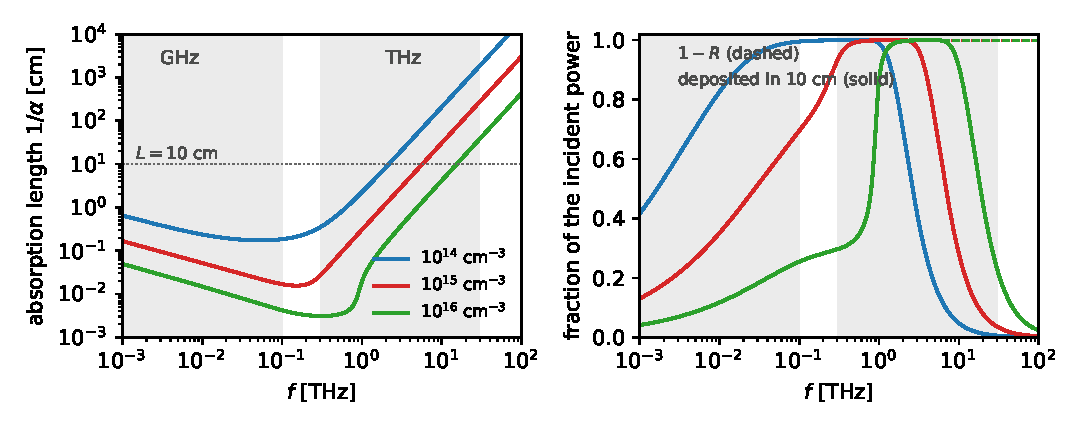
\includegraphics[width=0.86\textwidth]{fig_v5.pdf}
\caption{Pure Kr at 0.5~atm. Left: the absorption length against frequency for the three
densities, with the depth $L=10$~cm dotted; the shaded bands are the GHz range (1 to 100~GHz) and
the THz range (0.3 to 30~THz). Right: the fraction of the incident power that enters the gas,
$1-R$ (dashed), and the fraction deposited in the 10~cm (solid).}
\label{fig:spectrum}
\end{figure}

{\noindent}(3) \emph{GHz.} At $10^{15}$ and $10^{16}$~cm$^{-3}$ the gas is a mirror: it reflects 31
to 94\,\% between 2.45 and 95~GHz at 0.5~atm, 8 to 96\,\% over all pressures, and absorbs the
remainder within 0.04 to 1.1~mm of the front. At $10^{14}$~cm$^{-3}$ the collisions outrun the
cutoff and the wave gets in (43\,\% reflected at 2.45~GHz and 1\,\% at 95~GHz), but it is absorbed
in 1.8 to 4.2~mm (0.6 to 8.3~mm over the pressures and both gases): the front millimetres take
all of it and the rest of the gas nothing, since the deposition falls by $e^{\alpha L}$, at least
$10^{5}$, from front to back. \\ \\
\emph{THz.} The gas reflects at most 15\,\% (1~THz at
$10^{16}$~cm$^{-3}$) and nothing above 3~THz, and the absorption length runs from 0.2~mm to 2~m,
through the depth of the gas at 2.2, 5.7 and 15.4~THz for the three densities at 0.5~atm, and at
1.1 to 26.5~THz over the 18 cells. At 3~THz the 10~cm deposits 41, 97 and 100\,\% of the incident
power. Per electron the heating at a given intensity goes as $\nueff/(\omega^2+\nueff^2)$ by
Eq.~\eqref{eq:P-drude}, largest at GHz, where every electron heats as in a static field, and that
is exactly why the skin is thin: the first electrons take the whole wave. The GHz range would be
the right one only for a gas a millimetre thick at $10^{14}$~cm$^{-3}$ and 0.5~atm or more, where
95~GHz enters with 1\,\% reflection and is absorbed in 1.8 to 5.4~mm, or at densities below
$10^{12}$~cm$^{-3}$, where the cutoff falls to 9~GHz. Kr/F$_2$ changes the absorption lengths by at
most a factor 1.3 at 95~GHz and 3~THz and the reflections by at most 9 points.

\medskip
\noindent\textbf{In Summary:} For a gas deeper than a few millimetres the THz range is better: it
enters the gas and deposits over centimetres, where the GHz range reflects or skins. The best
frequency of Eq.~\eqref{eq:fA} lies on the transparent side of the peak, in the THz range at every
cell.


%================================================================
\section{The two gases}
\label{sec:results}
%================================================================

\subsection{The best frequencies}
\label{sec:table}
Table~\ref{tab:main} gives $\fbest$ at $L=10$~cm and 300~kW/cm$^3$ for the two gases,
with $\Te$ from Eq.~\eqref{eq:balance}. The flags come from the particle balance of
Sec.~\ref{sec:particles}.

\begin{table}[ht]
\centering
\caption{The best frequency in THz at $L=10$~cm and 300~kW/cm$^3$, with $\Te$ in eV in
parentheses, for the two gases. $^a$: the field's own ionization outruns the losses and
$n_e$ grows during the pulse. $^s$: the losses outrun it and a source must hold $n_e$.}
\label{tab:main}
\begin{tabular}{lccc}
\toprule
$n_e$ [cm$^{-3}$] & 0.1 atm & 0.5 atm & 2 atm\\
\midrule
\multicolumn{4}{l}{\emph{pure Kr}}\\
\tabinput{tab_envelope_v4_Kr.tex}
\addlinespace
\multicolumn{4}{l}{\emph{Kr + 2\,\% F$_2$}}\\
\tabinput{tab_envelope_v4_KrF2.tex}
\bottomrule
\end{tabular}
\end{table}

\subsection{The particle balance}
\label{sec:particles}
{\noindent}(1) The density is not the field's to choose. Direct ionization by the
electrons, at the rate $\nu_{\rm ion}=N\sum_jx_jk_{{\rm ion},j}$ from the thresholds at
14.0~eV (Kr) and 15.7~eV (F$_2$), makes electrons. Attachment to F$_2$ at
$\nu_{\rm att}=Nx_{{\rm F}_2}k_{\rm att}$ removes them, and so does recombination. For the
recombination every cation is taken as Kr$_2^+$ with the coefficient of Shiu and Biondi
\cite{ShiuBiondi1977},
\begin{equation}
\alpha_{\rm rec}=1.6\times10^{-6}\Big(\frac{300~{\rm K}}{\Te}\Big)^{0.55}~{\rm cm^3/s},\qquad
\nu_{\rm rec}=\alpha_{\rm rec}\,n_e,
\label{eq:rec}
\end{equation}
measured from 300 to 8400~K, 0.72~eV, and extrapolated here. The net rate is
$\nu_{\rm net}=\nu_{\rm ion}-\nu_{\rm att}-\nu_{\rm rec}$.
\\ \\
{\noindent}(2) Where $\nu_{\rm net}>0$ the density e-folds in $1/\nu_{\rm net}$, which is 2.4
to 5.2~ns at the four cells marked $^a$ (pure Kr at $10^{14}$~cm$^{-3}$, and Kr/F$_2$ at
$10^{14}$~cm$^{-3}$ and 0.1~atm). Where $\nu_{\rm net}<0$ a source must supply
$-\nu_{\rm net}n_e$ electrons per second, at the least at the ionization energy of krypton,
\begin{equation}
\boxed{\;P_{\rm src}\ge n_e\,(\nu_{\rm att}+\nu_{\rm rec}-\nu_{\rm ion})\times14.0~{\rm eV}.\;}
\label{eq:Psrc}
\end{equation}
In pure Kr, where recombination is the loss, that is 300 to 410~kW/cm$^3$ at $10^{15}$ and
41 to 49~MW/cm$^3$ at $10^{16}$~cm$^{-3}$. With 2\,\% F$_2$ the loss is attachment at
$5.8\times10^{7}$ to $1.3\times10^{10}$~s$^{-1}$, and the source needs 32 and 430~kW/cm$^3$ at
$10^{14}$~cm$^{-3}$ and 0.5 and 2~atm, 0.5 to 7.8~MW/cm$^3$ at $10^{15}$ and 46 to
470~MW/cm$^3$ at $10^{16}$~cm$^{-3}$. Neither gas holds $10^{16}$~cm$^{-3}$ at these powers,
and Kr/F$_2$ does not hold $10^{15}$ either.
\\ \\
{\noindent}(3) Pure Kr left to itself settles where its ionization balances
recombination, $\nu_{\rm ion}(\Te(P/n_e))=\alpha_{\rm rec}(\Te)\,n_e$, in $1/\nu_{\rm ion}=15$
to 19~ns: at $n_e=4.5$, 3.6 and $2.9\times10^{14}$~cm$^{-3}$ for 0.1, 0.5 and 2~atm
($\Te=2.0$, 1.6 and 1.4~eV), where $\fbest=2.1$, 3.7 and 6.1~THz. Over 100 to
500~kW/cm$^3$ that is $1.6$ to $6\times10^{14}$~cm$^{-3}$ and 1.5 to 7.2~THz.

\subsection{The power laws}
\label{sec:laws}
Fitted to the nine cells of each gas at 300~kW/cm$^3$,
\begin{equation}
\boxed{\;\fbest\approx C\,\Big(\frac{n_e}{10^{15}~{\rm cm^{-3}}}\Big)^{b}
\Big(\frac{p}{1~{\rm atm}}\Big)^{c}\Big(\frac{L}{10~{\rm cm}}\Big)^{1/2},\;}
\label{eq:law}
\end{equation}
with $C=7.6$~THz, $b=0.43$, $c=0.40$ for pure Kr within 5.1\,\%, and $C=7.1$~THz, $b=0.41$,
$c=0.37$ for Kr/F$_2$ within 8.6\,\%. From 100 to 500~kW/cm$^3$ the best frequency rises by at most a
factor 1.16 in pure Kr, through $\Te$: at $10^{15}$~cm$^{-3}$ and 0.5~atm it is 4.4, 7.1 and
8.7~THz for $\Te=1$, 2 and 4~eV. In Kr/F$_2$ the power moves it by up to a factor 3.4, at
$10^{15}$~cm$^{-3}$ and 2~atm, since at 100~kW/cm$^3$ the F$_2$ losses already hold the
electrons at 0.16~eV there.

\subsection{Fluorine against pure krypton}
\label{sec:f2}
{\noindent}(1) At a given $\Te$ the 2\,\% F$_2$ adds at most 4.6\,\% to the kernel \eqref{eq:nuea}, so
the frequency is the same wherever the krypton excitation takes the power: Kr/F$_2$ is within 2\,\%
of pure Kr at six cells ($\Te\ge1.2$~eV) and 9 to 18\,\% below it at $10^{15}$~cm$^{-3}$ and 2~atm and
at $10^{16}$~cm$^{-3}$ and 0.5 and 2~atm, where the F$_2$ losses hold the electrons in the Ramsauer
minimum.
\\ \\
{\noindent}(2) What F$_2$ changes is the closure. Attachment removes the electrons in 0.1 to 17~ns,
so a source must hold the density nearly everywhere, and from $10^{15}$~cm$^{-3}$ up the source's
power exceeds the field's and its electrons set $\Te$ (Secs.~\ref{sec:kinetic} and
\ref{sec:uncertainty}).

\medskip
\noindent\textbf{In Summary:} Pure Kr wants 1.1 to 3.8~THz at $10^{14}$~cm$^{-3}$, 3.0 to
10.1 at $10^{15}$ and 8.7 to 26.5~THz at $10^{16}$, and 2\,\% F$_2$ changes the frequency only where
its losses cool the electrons. The density is the source's choice wherever F$_2$ is present, and
neither gas holds $10^{16}$~cm$^{-3}$ at these powers.


%================================================================
\section{The kinetic check}
\label{sec:kinetic}
%================================================================
{\noindent}(1) The envelope takes the electrons as Maxwellian. A two-term kinetic
solution \cite{HP2005} of every cell, with the same cross sections, the elastic collisions
with the ions, electron--electron collisions in Landau's form, and the temporal-growth
model in which the electrons that attachment removes or ionization adds are replaced or
removed with the shape of the distribution, gives $\Te$ as two thirds of the mean energy
and the absorption from the complex mobility at the envelope's $\fbest$, from which the
kinetic $f_A$ follows with $\alpha\propto f^{-2}$.
\\ \\
{\noindent}(2) In pure Kr the kinetic $\Te$ is 0.94 to 1.35 times the envelope's and the
kinetic $\fbest$ 0.89 to 1.23 times it: the inelastic collisions deplete the tail that a
Maxwellian keeps, so the bulk must be hotter to lose the same power, most at
$10^{15}$~cm$^{-3}$. With 2\,\% F$_2$ the same holds at the four cells where the field
outweighs attachment, with $\fbest$ at 0.96 to 1.12 times the envelope. At the other five,
$10^{15}$~cm$^{-3}$ from 0.5~atm up and all of $10^{16}$, attachment takes 0.6 to 25 times the
field's power from the electrons, so the source that replaces them sets $\Te$, and the
growth model is no longer a field-heated plasma.

\medskip
\noindent\textbf{In Summary:} The Maxwellian envelope is good to $-11$ to $+23$\,\% in
frequency where the field sets the temperature. Where the source does, the temperature,
and with it the frequency, is the source's.


%================================================================
\section{The uncertainty of the result}
\label{sec:uncertainty}
%================================================================

\subsection{Propagation}
\label{sec:propagation}
{\noindent}(1) From Eq.~\eqref{eq:fA}, $\fbest\propto\nueff^{1/2}$, so that a fractional
change of the collision frequency moves the frequency by half of it, and a change of the
ions' term alone by half of its share $s_i=\nuei/\nueff$:
\begin{equation}
\boxed{\;\frac{\delta\fbest}{\fbest}=\frac12\,\frac{\delta\nueff}{\nueff},\qquad
\frac{\delta\fbest}{\fbest}=\frac{s_i}{2}\,\frac{\delta\nuei}{\nuei}.\;}
\label{eq:propagation}
\end{equation}
A change of $\Te$ acts through $\sigma_m(\Te)$: between 1 and 2~eV in pure Kr,
$\fbest\propto\Te^{0.70}$, and between 2 and 4~eV, $\Te^{0.31}$.
\\ \\
{\noindent}(2) Each cell gets a central value and one uncertainty, $\fbest\pm\delta$. With
the bands $[m_-,m_+]$, $[i_-,i_+]$, $[e_-,e_+]$ and $[x_-,x_+]$ of the four sources below
as factors on the envelope's value $f_{\rm env}$,
\begin{equation}
\boxed{\;\begin{aligned}
f_c&=f_{\rm env}\,\frac{m_-+m_+}{2}\,\frac{i_-+i_+}{2},\\
\frac{\delta}{f_c}&=\Big[\Big(\frac{m_+-m_-}{2}\Big)^2+\Big(\frac{i_+-i_-}{2}\Big)^2
+\Big(\frac{e_+-e_-}{2}\Big)^2+\Big(\frac{x_+-x_-}{2}\Big)^2\Big]^{1/2},
\end{aligned}\;}
\label{eq:delta}
\end{equation}
the half-widths added in quadrature as independent errors.

\subsection{The sources}
\label{sec:sources}
{\noindent}(M) \emph{The envelope against the kinetic solution.} The two models of
Sec.~\ref{sec:kinetic} bracket the answer: $m_\mp$ are the smaller and the larger of 1
and $f_{\rm kin}/f_{\rm env}$. The half-width is 0.2 to 12\,\% in pure Kr. At the five
source-set cells of Kr/F$_2$ the band is instead $\fbest$ over $\Te=1$ to 4~eV, 0.79 to 2.5
times the envelope, and its half-width, 27 to 62\,\%, stands in for (M).
\\ \\
{\noindent}(I) \emph{The electron--ion term against the measurements.} Turnbull et al.\
measured absorption fractions of 1 to 4\,\% in hydrogen and nitrogen--hydrogen plasmas
with an absolute uncertainty of ($-0.12$\,\%, $+0.07$\,\%), found their best shots
predicted to better than 10\,\%, and their models 16\,\% above the data on average without
the fitted screening factor \cite{Turnbull2023,Turnbull2024}. The electron--ion
absorption of Eqs.~\eqref{eq:nuT} and \eqref{eq:Lambda}, with the dynamic cutoff and the
exact Gaunt factor and no fitted factor, is 1.19 to 1.20 times their four hydrogen
measurements. Taking the measurements as right within 10\,\%, the ion term is 0.75 to
0.92 of the computed one, and Eq.~\eqref{eq:propagation} with the midpoint 0.84 gives
$i_\mp$: the half-width is 0.0 to 1.0\,\% in pure Kr, the most at $10^{16}$~cm$^{-3}$ and
0.1~atm, and up to 4.3\,\% at the cold cells, where the ions carry most of the absorption.
\\ \\
{\noindent}(E) \emph{The momentum-transfer cross section against swarm experiments.} The
atoms carry the absorption, so the cross section $\sigma_m$ of krypton is the input that matters,
and the electron drift velocity $W$ in a DC field is its experimental test: for $\omega\gg\nu$ the
absorption weights $\sigma_m$ as Eq.~\eqref{eq:nuea} does, and the drift velocity weights
$1/\sigma_m$ over the same electron energies, so that $\delta W/W\simeq-\delta\sigma_m/\sigma_m$. The
two-term equation \cite{HP2005} with the same Biagi set gives $W$ at each field strength of two
measurements in pure krypton, Pack, Voshall and Phelps \cite{Pack1962} at 300~K, as compiled by
Dutton \cite{Dutton1975}, and Nakamura \cite{Nakamura1991}, read from the figure of the published
abstract to about 3\,\%. Each measured point is placed at the electron temperature
$\Te=\tfrac23\langle\varepsilon\rangle$ of the computed swarm. Between 0.95 and 2.6~eV, the range of the
warm cells, the computed $W$ is 0.96 to 1.02 times Nakamura's (rms 1.8\,\%, 13 points) and 0.84
to 0.97 times Pack's (rms 8.4\,\%, 7 points), and the two experiments differ from each other by
as much. Below that range only Pack's data exist, and across the Ramsauer minimum the computed
$W$ is 0.80 to 1.20 times them. For each cell the points within $\pm25$\,\% of its $\Te$ give the
rms deviation of each experiment, and their quadratic mean $d$ weights the two experiments
equally. Since only the atoms' share $1-s_i$ of $\nueff$ depends on $\sigma_m$, and
$\fbest\propto\nueff^{1/2}$, the half-width is
\begin{equation}
\boxed{\;\frac{e_+-e_-}{2}=(1-s_i)\,\frac d2,\;}
\label{eq:swarm}
\end{equation}
1.4 to 4.0\,\% in pure Kr. The same deviation, taken as an uncertainty of $\sigma_m$, replaces an
assumed one: had $\sigma_m$ been taken as good to 10\,\%, Eq.~\eqref{eq:propagation} and the cells
recomputed with $\sigma_m\times0.9$ and $\times1.1$ give 3.7 to 5.0\,\% in pure Kr. Adding both would
count the cross section twice, so Eq.~\eqref{eq:delta} carries (E), and the 10\,\% figure stands as
a bound that the swarm data do not reach.

{\noindent}(X) \emph{The inelastic cross sections of krypton}, taken as good to 20\,\%,
move $\Te$ through Eq.~\eqref{eq:balance} and with it $\fbest$ by 1.0 to 1.7\,\% in pure Kr.

{\noindent}(D) \emph{The recombination coefficient}, $\pm10$\,\% as stated
\cite{ShiuBiondi1977}, moves the self-sustained density of pure Kr by $-4.0$ to $+4.6$\,\%
and its frequency by $\mp1.9$\,\%. Its extrapolation beyond 0.72~eV is not bounded.

\subsection{The result}
\label{sec:uresult}
Table~\ref{tab:uncert} gives $\fbest\pm\delta$ at the 18 cells with the four contributions.
In pure Kr $\delta/\fbest$ is 2 to 12\,\%, and (M) and (E) together carry most of $\delta^2$ at eight
of the nine cells. In Kr/F$_2$ it is 3 to
7\,\% at the four field-set cells and 27 to 62\,\% at the five source-set ones, where the
temperature the source chooses is the uncertainty.

{\small
\setlength{\tabcolsep}{4pt}
\begin{longtable}{llccccccc}
\caption{The best frequency with its uncertainty at every cell of Table~\ref*{tab:main},
and the four contributions to $\delta$ in per cent. $^t$: the source sets $\Te$, and the
half-width of $\fbest$ over $\Te=1$ to 4~eV stands in for (M).}\label{tab:uncert}\\
\toprule
gas & $n_e$ [cm$^{-3}$] & $p$ [atm] & $\fbest\pm\delta$ [THz] & $\delta$ [\%] & (M) & (I) & (E) & (X)\\
\midrule
\endfirsthead
\toprule
gas & $n_e$ [cm$^{-3}$] & $p$ [atm] & $\fbest\pm\delta$ [THz] & $\delta$ [\%] & (M) & (I) & (E) & (X)\\
\midrule
\endhead
\bottomrule
\endfoot
\tabinput{tab_uncert_v6.tex}
\end{longtable}}

\medskip
\noindent\textbf{In Summary:} The uncertainty of the best frequency is
Eq.~\eqref{eq:delta} from the Maxwellian envelope against the kinetic solution, the
electron--ion term against Turnbull's data, the momentum-transfer cross section against the
swarm measurements, and the inelastic cross sections. It is 2 to 12\,\% in pure Kr, since the
atoms carry the absorption, their cross section reproduces the measured drift velocities to a
few per cent, and the ion term that Turnbull's measurements test contributes at most 1\,\%, and it is the source's temperature wherever F$_2$ makes a
source necessary.


%================================================================
\section{A worked example}
\label{sec:example}
%================================================================
Pure Kr at $n_e=10^{15}$~cm$^{-3}$, $p=0.5$~atm, $P=300$~kW/cm$^3$ and $L=10$~cm, the central cell
of Table~\ref{tab:main}, carried through from the gas density to the recommended frequency.
\\ \\
{\noindent}(1) \emph{The gas and the power per electron.} $N=2.45\times10^{19}\times0.5=1.22\times10^{19}$
atoms per cm$^3$, and $P/n_e=3\times10^{5}~{\rm W\,cm^{-3}}/10^{15}~{\rm cm^{-3}}=1.87\times10^{9}$~eV/s
per electron.
\\ \\
{\noindent}(2) \emph{The temperature.} Equation~\eqref{eq:balance} balances at $\kB\Te=1.42$~eV:
the recoil of Eq.~\eqref{eq:Pel} takes $3.3\times10^{7}$~eV/s, 1.8\,\%, and krypton's levels take
$1.84\times10^{9}$~eV/s, the rest.
\\ \\
{\noindent}(3) \emph{The collision frequency.} The kernel \eqref{eq:nuea} gives
$\nuea=1.22\times10^{12}$~s$^{-1}$, 2.10 times the Drude mean $5.8\times10^{11}$~s$^{-1}$. For the
ions, Eq.~\eqref{eq:nuT} gives $\nuT=1.71\times10^{9}$~s$^{-1}$, $\eta_t=4.4$ puts the collisions in
the classical regime, $\Lambda=3.65$ where the Born logarithm would give 4.90, and
$\nuei=6.3\times10^{9}$~s$^{-1}$, 0.5\,\% of $\nueff=1.22\times10^{12}$~s$^{-1}$. So
$\nueff/2\pi=0.19$~THz.
\\ \\
{\noindent}(4) \emph{The cutoff and the reflection limit.} $f_{pe}=8.98~{\rm kHz}\times(10^{15})^{1/2}
=0.28$~THz, and $f_R=1.294f_{pe}=0.37$~THz without the collisions, 0.32~THz with them in
Eq.~\eqref{eq:optics}.
\\ \\
{\noindent}(5) \emph{The absorption length.} Equation~\eqref{eq:fA} with $n_e/10^{15}=1$,
$\nueff/10^{12}=1.22$ and $L/10~{\rm cm}=1$ gives $f_A=5.2\times(1.22)^{1/2}=5.73$~THz, and the exact
root of $\alpha L=1$ is 5.73~THz. So $\fbest=5.7$~THz, far above $f_R$. There $u=0.017$ and
$\alpha_L=2.2\times10^{-3}$, so the soft-photon kernel and the absence of Langdon's flattening both
hold.
\\ \\
{\noindent}(6) \emph{The field.} Equation~\eqref{eq:E0} gives $E_0=47.6$~kV/cm, an intensity of
3~MW/cm$^2$.
\\ \\
{\noindent}(7) \emph{GHz instead?} At 95~GHz, $\nueff/\omega=2.1$: the wave is in the collisional
skin, with an absorption length of 0.17~mm and 31\,\% reflected. At 2.45~GHz, 1.1~mm and 80\,\%
reflected. At 1~THz the gas is already transparent, $R=0$, but the absorption length is 3.0~mm and
the front centimetre takes everything. At 3~THz it is 2.7~cm. The depth of the gas is matched on
the transparent side, at 5.7~THz.
\\ \\
{\noindent}(8) \emph{The density.} Direct ionization runs at $\nu_{\rm ion}=1.6\times10^{7}$~s$^{-1}$
against recombination at $1.8\times10^{8}$~s$^{-1}$ (5.7~ns per electron), so this density decays
unless a source supplies at least 360~kW/cm$^3$ by Eq.~\eqref{eq:Psrc}, more than the field. Left to
itself at this pressure and power, pure Kr settles at $3.6\times10^{14}$~cm$^{-3}$ and
$\kB\Te=1.62$~eV in 17~ns, where $\fbest=3.7$~THz.
\\ \\
{\noindent}(9) \emph{The uncertainty.} The kinetic solution of Sec.~\ref{sec:kinetic} gives
$\kB\Te=1.80$~eV and $\fbest=6.7$~THz, 1.17 times the envelope, so (M) contributes a half-width
of 8.7\,\%; (I) 0.02\,\%, since the ions carry 0.5\,\%; (E) 1.7\,\%, from the 9 swarm points within
$\pm25$\,\% of 1.42~eV, where the computed drift velocity deviates from Nakamura's by 1.2\,\% rms and
from Pack's by 4.6\,\%, so that $d=3.3\,\%$; (X) 1.7\,\%. Equation~\eqref{eq:delta} gives
$\delta/\fbest=9.0\,\%$ about the midpoint:
\begin{equation}
\boxed{\;\fbest=6.2\pm0.6~{\rm THz}.\;}
\label{eq:example}
\end{equation}
\\ \\
{\noindent}(10) \emph{With 2\,\% F$_2$ at the same point.} $\kB\Te=1.37$~eV, F$_2$'s channels taking
26\,\% of the losses, and $\fbest=5.6$~THz, 2\,\% below pure krypton's. But attachment runs at
$6.1\times10^{8}$~s$^{-1}$, 1.6~ns per electron, the source must supply at least 1.7~MW/cm$^3$, six
times the field's power, and in the kinetic solution it takes 0.60 of the field's power from the
electrons, so it sets $\Te$ and the frequency is $6.6\pm2.5$~THz, 38\,\%.

\medskip
\noindent\textbf{In Summary:} At $10^{15}$~cm$^{-3}$, 0.5~atm and 300~kW/cm$^3$ in a 10~cm gas, the
best frequency is $6.2\pm0.6$~THz, Eq.~\eqref{eq:example}. The GHz range is out: 31 to 80\,\%
reflected and the rest absorbed in 0.2 to 1~mm. The density is not free: pure Kr at this
density needs a source of 360~kW/cm$^3$ or settles at $3.6\times10^{14}$~cm$^{-3}$, where it wants
3.7~THz, and with F$_2$ the source needs 1.7~MW/cm$^3$ and sets the temperature.


%================================================================
\section{Summary}
\label{sec:summary}
%================================================================
\noindent\textbf{In Summary:} The best frequency for inverse-bremsstrahlung heating of a
krypton laser gas is the one whose absorption length matches the depth of the gas,
Eq.~\eqref{eq:fbest}, and it is Eq.~\eqref{eq:fA}: the square root of the electron
density, of the collision frequency and of the depth. The collision frequency is that of
the atoms, Eq.~\eqref{eq:nuea}, which the ions supplement by a few per cent at
$10^{15}$~cm$^{-3}$ and by up to a quarter at $10^{16}$, and it depends on the electron
temperature that the power balance \eqref{eq:balance} sets, 0.95 to 2.6~eV where the
field sets it. Pure Kr wants $1.1\pm0.1$~THz at $10^{14}$~cm$^{-3}$ and 0.1~atm, rising as
$(n_ep)^{0.4}$ and $L^{1/2}$ to $27.9\pm1.7$~THz at $10^{16}$~cm$^{-3}$ and 2~atm, with 2 to
12\,\% uncertainty, and left to itself it runs at $1.6$ to $6\times10^{14}$~cm$^{-3}$ and
wants 1.5 to 7~THz. The THz range is the right one: across the spectrum the absorption
peaks at 0.05 to 0.50~THz, between the bands, and the GHz range either reflects, 31 to 94\,\%
from $10^{15}$~cm$^{-3}$ up, or is absorbed in a millimetre skin, while the THz range enters the
gas and deposits over centimetres. 2\,\% F$_2$ leaves the frequency alone wherever the
krypton excitation takes the power. But F$_2$ attaches the electrons in 0.1 to 17~ns, so a
source sets the density and, from $10^{15}$~cm$^{-3}$ up, the temperature, and the frequency
is then known only to the source's temperature, 27 to 62\,\%. Neither gas holds
$10^{16}$~cm$^{-3}$ at 100 to 500~kW/cm$^3$. At the worked example, pure Kr at
$10^{15}$~cm$^{-3}$ and 0.5~atm, the answer is $6.2\pm0.6$~THz.


\appendix
%================================================================
\section{The numerical checks}
\label{app:checks}
%================================================================
The script \texttt{envelope\_v6\_check.py} verifies every boxed result of these notes, in
their order, by an independent numerical route: the Drude optics against the exact
complex refractive index, the energy-weighted kernel \eqref{eq:nuea} against the
velocity-space integral \eqref{eq:nuea-general} by quadrature and against the $4/3$ of a
constant cross section, the rate \eqref{eq:rate} and the recoil loss \eqref{eq:Pel}
against quadrature and against the closed form of a step cross section, the Spitzer
prefactor, the Born and classical limits of the logarithm, the reflection limit
\eqref{eq:fR}, the closed form \eqref{eq:fA} against the exact root, the field
\eqref{eq:E0} and Langdon's parameter \eqref{eq:alphaL} against the solved cells, the
particle balance, the fits \eqref{eq:law}, the collisional-skin law \eqref{eq:skin}, the
swarm comparison \eqref{eq:swarm} with the drift velocities recomputed and the measured values read
from their data files, the combination \eqref{eq:delta}, and every step of the worked example of Sec.~\ref{sec:example}. It
reproduces every number printed in these notes to its last printed digit from the stored results
of \texttt{envelope\_v6.py} and \texttt{swarm\_kr.py}, checks the quoted figures of Turnbull et al.\ against the text of
their papers, and checks the logical statements. It runs with \texttt{numpy} and \texttt{scipy}
under \texttt{/usr/bin/python3} in a few seconds from those stored results, which the scripts
behind them take about four minutes to produce. Table~\ref{tab:checks} is
written by the script itself. A quantitative check passes when its deviation is below
the tolerance stated in the script, a printed number when the script reproduces it to
its last printed digit, and a logical condition when it holds.

% written by envelope_v6_check.py -- do not edit by hand
\begin{longtable}{L{4.0cm}cccc}
\caption{The numerical checks of \texttt{envelope\_v6\_check.py}, by the equation, table or section they verify. The second column counts all checks of the row. The third gives the largest deviation among its quantitative checks, relative, or absolute for quantities near zero, and is empty when the row has none. The fourth counts the numbers printed in these notes that the script reproduces to their last printed digit, and the fifth the logical conditions.}\label{tab:checks}\\
\toprule
Equation & Checks & Largest deviation & Printed & Logical\\
\midrule
\endfirsthead
\toprule
Equation & Checks & Largest deviation & Printed & Logical\\
\midrule
\endhead
\bottomrule
\endfoot
Sec.~\ref*{sec:question} & 2 &  & 1 & 1\\
Eq.~(\ref*{eq:fbest}) & 5 &  & 2 & 3\\
Eq.~(\ref*{eq:drude-eps}) & 2 & $0$ &  & 1\\
Eq.~(\ref*{eq:optics}) & 10 & $1.3\times10^{-9}$ & 6 & 2\\
Eq.~(\ref*{eq:alpha}) & 2 & $1.0\times10^{-4}$ &  & \\
Eq.~(\ref*{eq:P-drude}) & 1 & $0$ &  & \\
Eq.~(\ref*{eq:drude-sigma}) & 1 & $0$ &  & \\
Eq.~(\ref*{eq:nuea}) & 8 & $1.7\times10^{-7}$ & 5 & \\
Sec.~\ref*{sec:atoms} & 1 &  & 1 & \\
Eq.~(\ref*{eq:Pel}) & 4 & $1.7\times10^{-7}$ & 2 & 1\\
Eq.~(\ref*{eq:nuT}) & 5 & $1.3\times10^{-3}$ & 2 & \\
Eq.~(\ref*{eq:Lambda1}) & 3 & $1.1\times10^{-9}$ & 1 & \\
Eq.~(\ref*{eq:Lambda}) & 4 & $4.2\times10^{-3}$ & 1 & 1\\
Sec.~\ref*{sec:ions} & 7 & $2.7\times10^{-6}$ & 6 & \\
Eq.~(\ref*{eq:nueff}) & 12 &  & 9 & 3\\
Sec.~\ref*{sec:leftout} & 2 &  & 1 & 1\\
Eq.~(\ref*{eq:alphaL}) & 4 & $5.7\times10^{-2}$ & 2 & 1\\
Eq.~(\ref*{eq:balance}) & 6 & $1.3\times10^{-13}$ & 3 & 1\\
Eq.~(\ref*{eq:rate}) & 3 & $8.3\times10^{-5}$ &  & \\
Sec.~\ref*{sec:temperature} & 21 &  & 19 & 2\\
Eq.~(\ref*{eq:E0}) & 6 & $2.7\times10^{-10}$ & 4 & 1\\
Eq.~(\ref*{eq:fR}) & 10 & $1.0\times10^{-13}$ & 7 & 1\\
Sec.~\ref*{sec:reflection} & 2 &  & 1 & 1\\
Eq.~(\ref*{eq:fA}) & 8 & $2.2\times10^{-3}$ & 5 & 2\\
Sec.~\ref*{sec:spectrum} & 42 &  & 36 & 6\\
Eq.~(\ref*{eq:skin}) & 5 & $0$ & 3 & 1\\
Table~\ref*{tab:spectrum} & 10 &  &  & 10\\
Table~\ref*{tab:main} & 19 &  &  & 19\\
Eq.~(\ref*{eq:rec}) & 6 &  & 3 & 3\\
Sec.~\ref*{sec:particles} & 36 &  & 33 & 3\\
Eq.~(\ref*{eq:Psrc}) & 4 &  & 1 & 3\\
Eq.~(\ref*{eq:law}) & 9 & $0$ &  & 3\\
Sec.~\ref*{sec:laws} & 7 &  & 6 & 1\\
Sec.~\ref*{sec:f2} & 7 &  & 5 & 2\\
Sec.~\ref*{sec:summary} & 15 &  & 14 & 1\\
Sec.~\ref*{sec:results} & 1 &  &  & 1\\
Sec.~\ref*{sec:kinetic} & 16 &  & 13 & 3\\
Eq.~(\ref*{eq:propagation}) & 3 & $3.9\times10^{-3}$ & 2 & \\
Eq.~(\ref*{eq:delta}) & 11 &  & 8 & 3\\
Sec.~\ref*{sec:sources} & 29 &  & 21 & 8\\
Eq.~(\ref*{eq:swarm}) & 23 & $0$ & 11 & 8\\
Sec.~\ref*{sec:uresult} & 7 &  & 6 & 1\\
Table~\ref*{tab:uncert} & 19 &  &  & 19\\
Sec.~\ref*{sec:example} & 22 & $0$ & 16 & 4\\
Eq.~(\ref*{eq:example}) & 5 & $0$ & 2 & 1\\
Appendix~\ref*{app:checks} & 4 &  &  & 4\\
\midrule
Total & 429 & & 258 & 126\\
\end{longtable}



\addcontentsline{toc}{section}{References}
\begin{thebibliography}{99}
\raggedright
\bibitem{Atzeni2004} S.~Atzeni and J.~Meyer-ter-Vehn, \emph{The Physics of Inertial Fusion}
(Oxford University Press, Oxford, 2004), doi:\href{https://doi.org/10.1093/acprof:oso/9780198562641.001.0001}{10.1093/acprof:oso/9780198562641.001.0001}.
\bibitem{Pitchford2016} L.~C.~Pitchford \emph{et al.}, Plasma Process. Polym. \textbf{14}, 1600098 (2016),
doi:\href{https://doi.org/10.1002/ppap.201600098}{10.1002/ppap.201600098} (LXCat, Biagi-v7.1 database).
\bibitem{Morgan1992} W.~L.~Morgan, Plasma Chem. Plasma Process. \textbf{12}, 449 (1992),
doi:\href{https://doi.org/10.1007/BF01447254}{10.1007/BF01447254} (LXCat, SIGLO database).
\bibitem{HP2005} G.~J.~M.~Hagelaar and L.~C.~Pitchford, Plasma Sources Sci. Technol. \textbf{14}, 722 (2005),
doi:\href{https://doi.org/10.1088/0963-0252/14/4/011}{10.1088/0963-0252/14/4/011}.
\bibitem{Low1958} F.~E.~Low, Phys. Rev. \textbf{110}, 974 (1958),
doi:\href{https://doi.org/10.1103/PhysRev.110.974}{10.1103/PhysRev.110.974}.
\bibitem{KrollWatson1973} N.~M.~Kroll and K.~M.~Watson, Phys. Rev. A \textbf{8}, 804 (1973),
doi:\href{https://doi.org/10.1103/PhysRevA.8.804}{10.1103/PhysRevA.8.804}.
\bibitem{KarzasLatter1961} W.~J.~Karzas and R.~Latter, Astrophys. J. Suppl. \textbf{6}, 167 (1961),
doi:\href{https://doi.org/10.1086/190063}{10.1086/190063}.
\bibitem{vanHoof2014} P.~A.~M.~van~Hoof, R.~J.~R.~Williams, K.~Volk, M.~Chatzikos, G.~J.~Ferland, M.~Lykins,
R.~L.~Porter and Y.~Wang, Mon. Not. R. Astron. Soc. \textbf{444}, 420 (2014),
doi:\href{https://doi.org/10.1093/mnras/stu1438}{10.1093/mnras/stu1438}.
\bibitem{DawsonOberman1962} J.~Dawson and C.~Oberman, Phys. Fluids \textbf{5}, 517 (1962),
doi:\href{https://doi.org/10.1063/1.1706652}{10.1063/1.1706652}.
\bibitem{Turnbull2023} D.~Turnbull \emph{et al.}, Phys. Rev. Lett. \textbf{130}, 145103 (2023),
doi:\href{https://doi.org/10.1103/PhysRevLett.130.145103}{10.1103/PhysRevLett.130.145103}.
\bibitem{Turnbull2024} D.~Turnbull \emph{et al.}, Phys. Plasmas \textbf{31}, 063304 (2024),
doi:\href{https://doi.org/10.1063/5.0203446}{10.1063/5.0203446}.
\bibitem{Langdon1980} A.~B.~Langdon, Phys. Rev. Lett. \textbf{44}, 575 (1980),
doi:\href{https://doi.org/10.1103/PhysRevLett.44.575}{10.1103/PhysRevLett.44.575}.
\bibitem{Pack1962} J.~L.~Pack, R.~E.~Voshall and A.~V.~Phelps, Phys. Rev. \textbf{127}, 2084 (1962),
doi:\href{https://doi.org/10.1103/PhysRev.127.2084}{10.1103/PhysRev.127.2084}.
\bibitem{Dutton1975} J.~Dutton, J. Phys. Chem. Ref. Data \textbf{4}, 577 (1975),
doi:\href{https://doi.org/10.1063/1.555525}{10.1063/1.555525}.
\bibitem{Nakamura1991} Y.~Nakamura, Meeting Abstracts of the Physical Society of Japan, 1991 autumn meeting,
abstract 27p-ZA-3, p.~103 (1991), doi:\href{https://doi.org/10.11316/jpsgaiyoa.1991.4.0_103}{10.11316/jpsgaiyoa.1991.4.0\_103}.
\bibitem{ShiuBiondi1977} Y.-J.~Shiu and M.~A.~Biondi, Phys. Rev. A \textbf{16}, 1817 (1977),
doi:\href{https://doi.org/10.1103/PhysRevA.16.1817}{10.1103/PhysRevA.16.1817}.
\end{thebibliography}

\end{document}
